\chapter{Methodology and Design \label{sec:methodology}}
\todo[inline]{Implementation: how was your experiment/project accomplished? 
Include enough details of your method and tooling that someone can easily replicate your results.
}

% PRELUDE
This chapter contains the design decision and steps taken to complete the testbed creation and testing. The project can broken into the three main areas of hardware, software and digital signal processing. 

\section{Hardware \label{sec:hardware}}

\subsection{Software Defined Radio \label{sec: SDRdongle}}
The fundamental hardware aspect for this project is the Software Defined Radio (SDR), specifically, the SDR receiver module. \todo{ADD SECTION LABELS} As mentioned in section 2,4, software defined radio technology has been recently experienced decreasing costs and proliferation (CITE!!!). Broadly, the testbed was designed to accomodate a potential range of USB-A capable SDR modules, with the capability initially tested on a low cost and qualirt RTL-SDR to use as a benchmark, before progressing to later prototyping on higher end LimeSDR.

\vspace{0.5cm} \noindent 
\textbf{(i) RTL-SDR Prototyping}
The low cost RTL-SDR was chosen as the initial SDR module for testbed prototyping  due to its low cost and wide availability. The specifics of the RTL-SDR are stated in section 2.4 \todo{REF}, it was connected to the RPi5 and higher level M1 Mac along with a simple SMI antenna as seen in the figure below \ref*{fig:rtlSDR}. 

\begin{figure}[htbp]
    \centering
    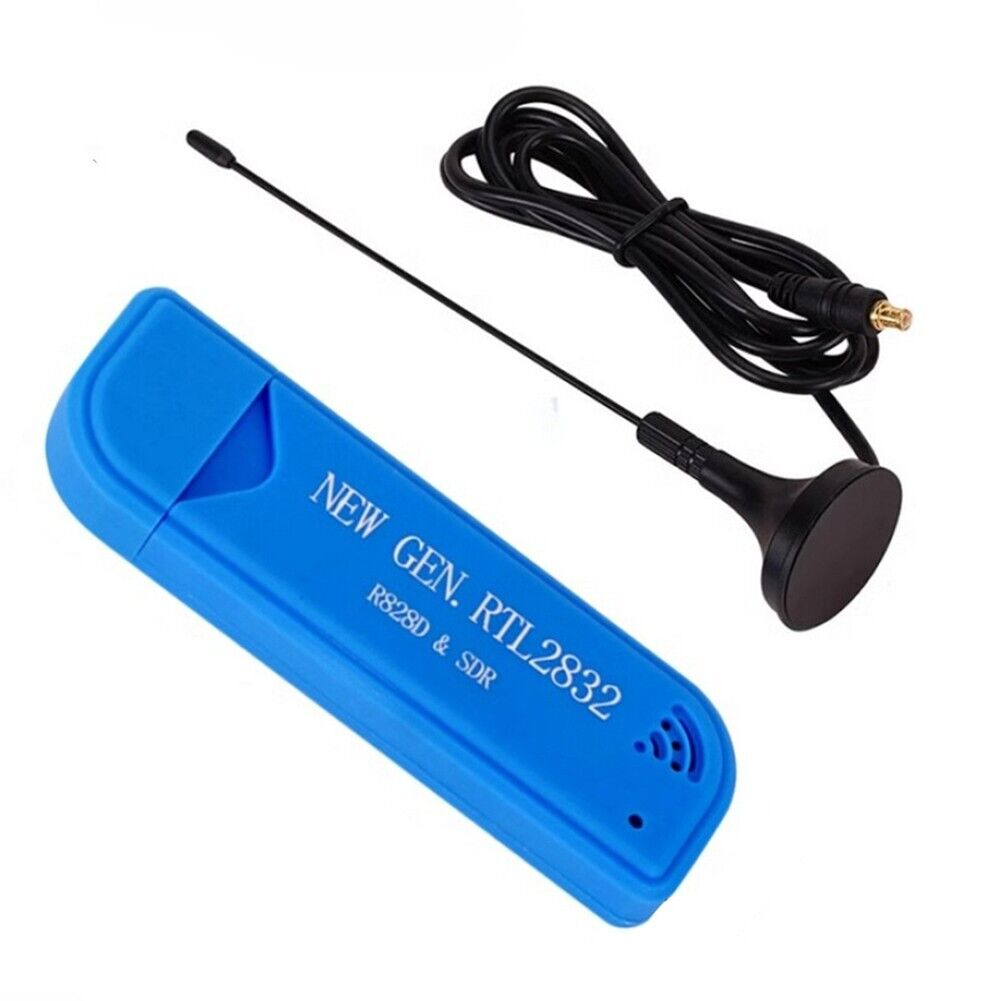
\includegraphics[width=0.3\textwidth]{rtlSdr.jpg}
    \caption{RTL-SDR with Simple SMA Antenna}
    \label{fig:rtlSDR}
\end{figure}

The RTL-SDR is based on the Realtek RTL2832U chipset, and has a frequency range of 24MHz to 1.7GHz, and a bandwidth of 3.2MHz. The RTL-SDR is also relatively cheap, with a price of around \$40 AUD, coming with compatibility to a wide range of software, including MATLAB, and GNU radio \cite{SDRdongle}. More specifically, the RTL-SDR was originally designed as a DVB-T receiver for digital TV, but due to its versatility, it has been repurposed by the hobbyist community for a wide range of RF signal reception applications. Fundamentally, the RTL-SDR is compised of two IC chips as seen in the block diagram figure below \ref*{fig:rtlSDRblock}; the RTL2832U, which is the digital TV demodulator, and the R820T, which is the tuner. The R820T is the chip that allows the RTL-SDR to tune to a wide range of frequencies, converting those signal frequencies to an intermediate baseband frequency which is processed by the RTL2832U. Inside the RTL2832U, the signal is then digitized and demodulated and sent to the host computer via USB.

\begin{figure}[htbp]
    \centering
    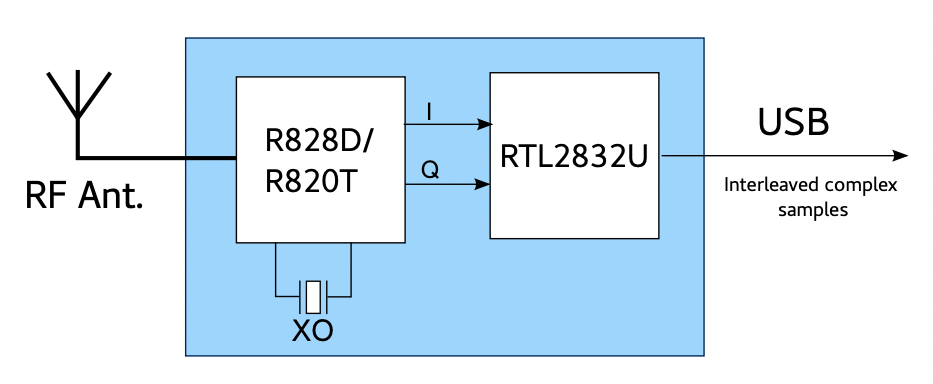
\includegraphics[width=0.7\textwidth]{rtlSDRchips.png}
    \caption{RTL-SDR Block Diagram \cite{RTLsdrBlockDiagram}}
    \label{fig:rtlSDRblock}
\end{figure}

\par \noindent
The RTL-SDR was tested with a range of software as mentioned in \ref*{sec:SDRsoftware} to ensure hardware was correctly functioning and to gain familiarity with the process. Specifically, given the nature of the digital signals utilised in this project, it was tested at the appropriate frequency range (approx 200Mhz). Furthemore, this was valuable to obtain ball park noise floor measurements, which eventuated to around -80dB when using the basic antenna. 

\vspace{0.5cm} \noindent 
\textbf{(ii) LimeSDR Implementation}
The LimeSDR was chosen as the higher end SDR module for the implementation and testing of the testbed. As seen in Table \ref{tab:SDRcomparison}, the LimeSDR has a frequency range of 100kHz to 3.8GHz, and a bandwidth of 61.44MHz. The LimeSDR is also more expensive than the RTL-SDR, with a price of around \$600 AUD. Specifically, the LimeSDR used was the LimeSDR-USB Version 1.4, which can be seen in the figure below \ref{fig:limeSDR}. 

\begin{figure}[htbp]
    \centering
    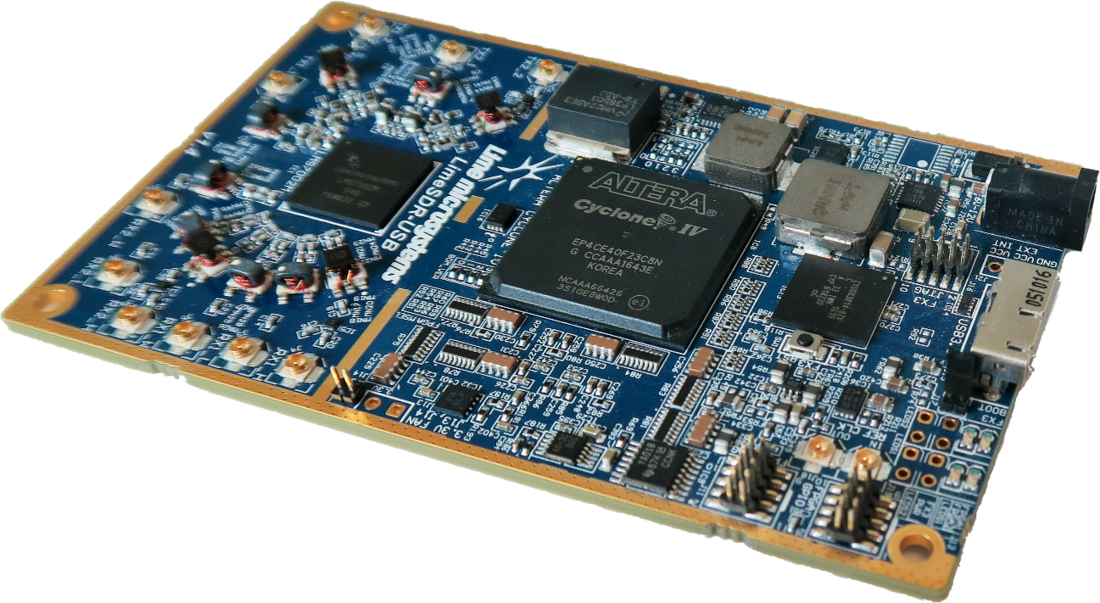
\includegraphics[width=0.5\textwidth]{limeSDR.png}
    \caption{LimeSDR-USB Version 1.4 PCB \cite{limesdr_usb}}
    \label{fig:limeSDR}
\end{figure}

The actual SDR module was encased as seen in XXX \todo{add photo in results}, with the only relevant conenctions being a singular RX SMA port, power supply (6V DC) and a USB type B connection. The block diagram of the LimeSDR can be seen in the figure below \ref{fig:limeSDRblock}, and evidently it is a more complex system than the RTL-SDR, most notably with the CycloneIV FPGA chip, which is used for signal processing and control.

\begin{figure}[htbp]
    \centering
    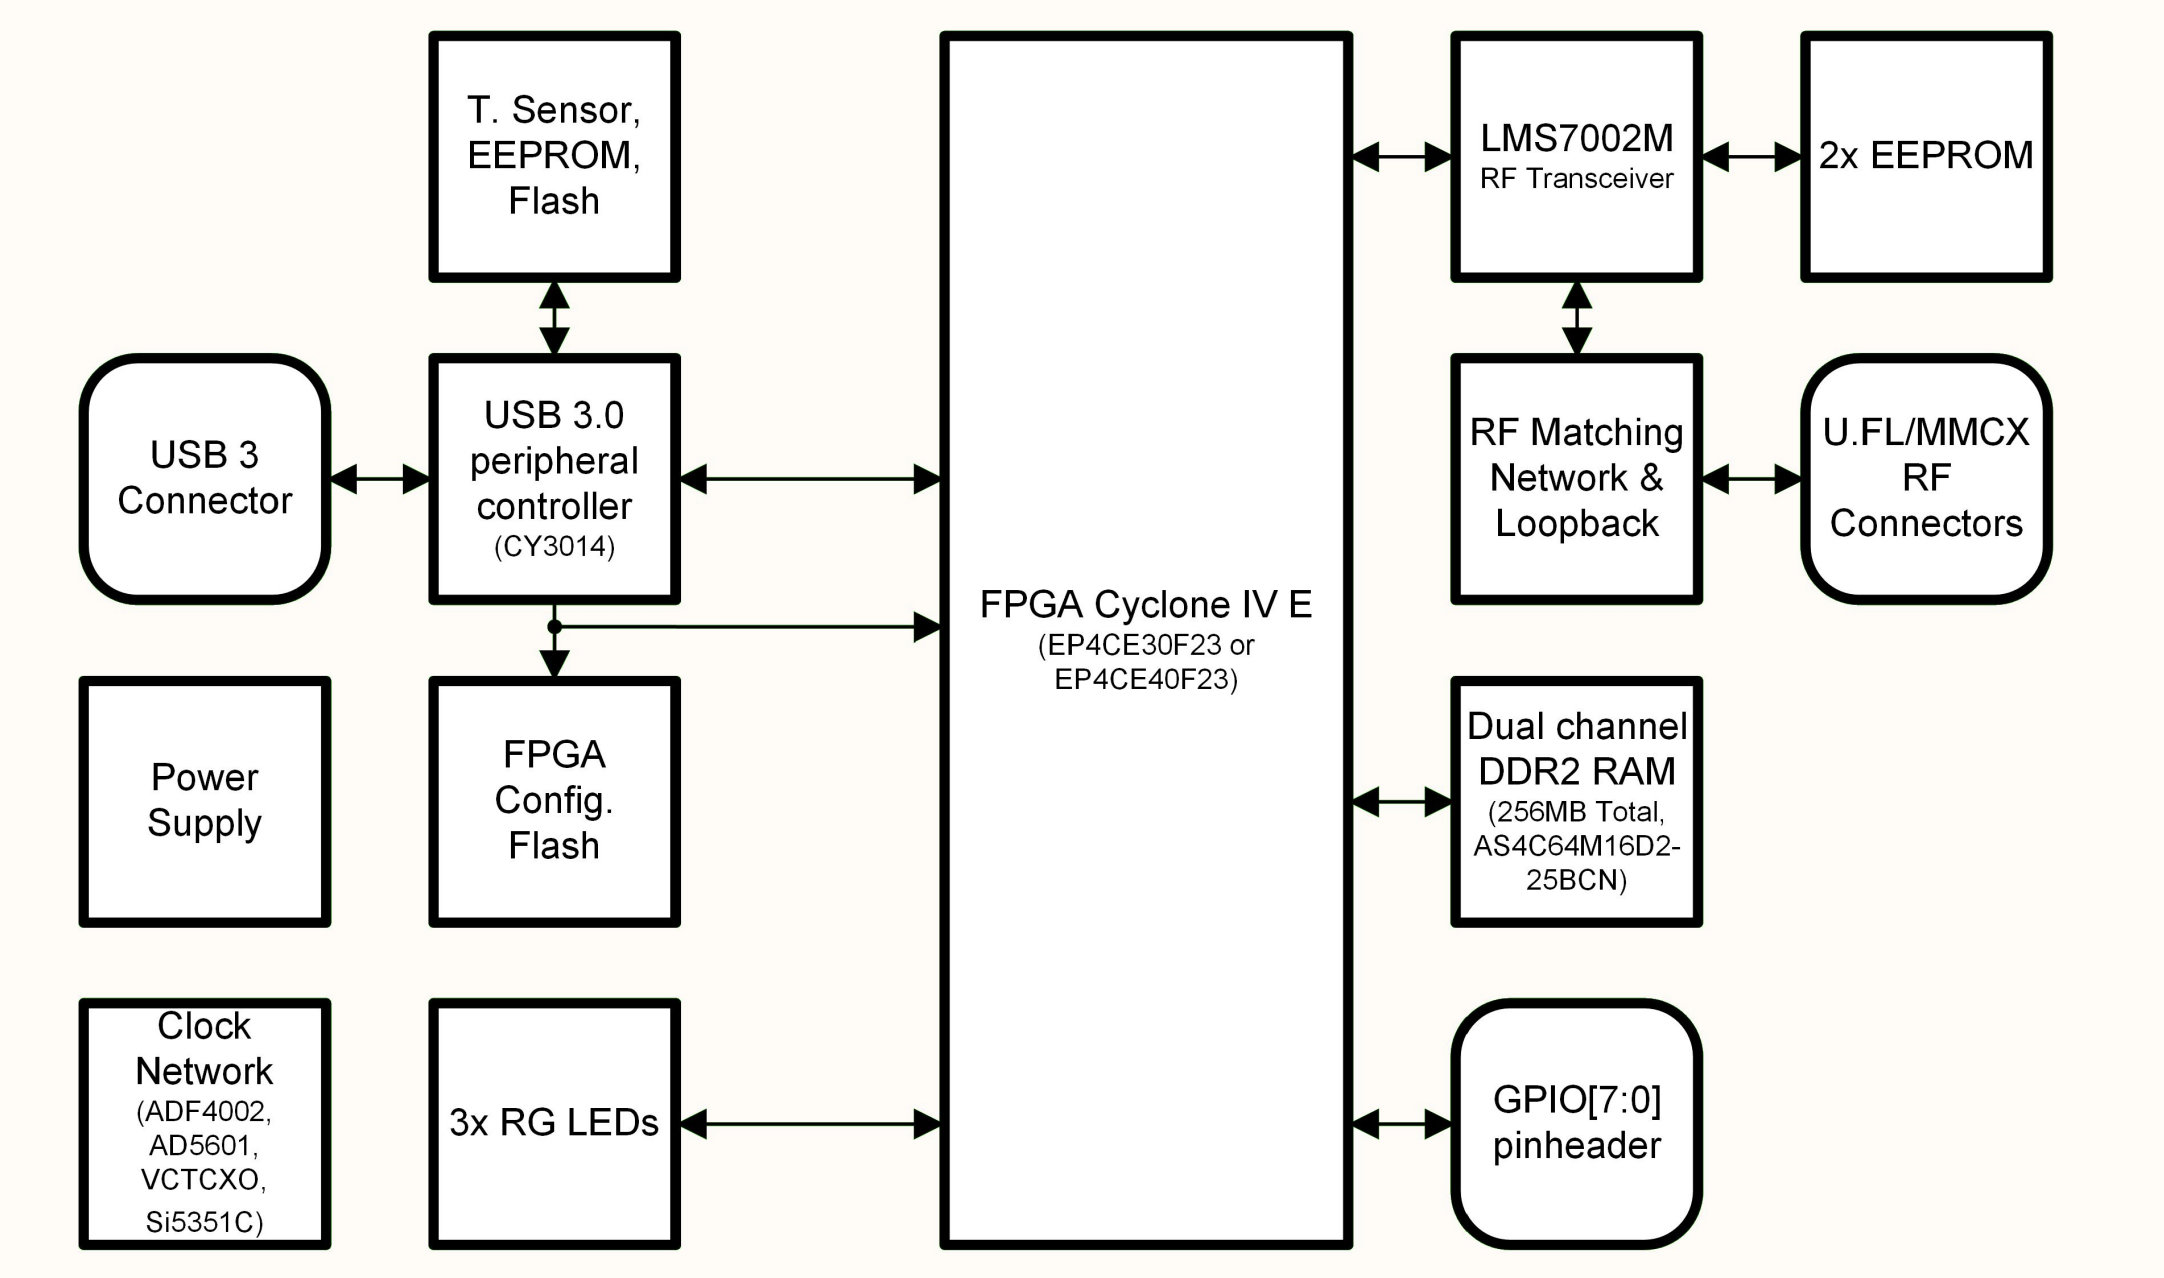
\includegraphics[width=0.7\textwidth]{limeSDRblock.png}
    \caption{LimeSDR Block Diagram \cite{limesdr_usb}}
    \label{fig:limeSDRblock}
\end{figure}

Another notable hardware feature of the LimeSDR is the LMS7002M transceiver chip which can facilitate both RX and TX capabilities, along with built in ADC/DAC (12 bit) capability \cite{limesdr_usb}. The bandwidth advantage of the LimeSDR was a key factor in its selection, as the wider bandwidth allows for more data to be captured and processed, specifically in the context of the digital broadcast signal used as the illuminator of opportunity. This bandwidth advantage directly results in increased range resolution on the range doppler maps, which is a key metric for the detection of aerial vehicles. \todo{Discuss USB 3.0 bottlneck, until X bandwidth samples/sec}


\subsection{Embedded Computing Platform \label{sec:embedded computing}}



The embedded computing platform chosen for the testbed was the Raspberry Pi 5 (RPi5), specifically the version with 8GB of RAM \cite{core_electronics_rpi5}. 

\begin{figure}[htbp]
    \centering
    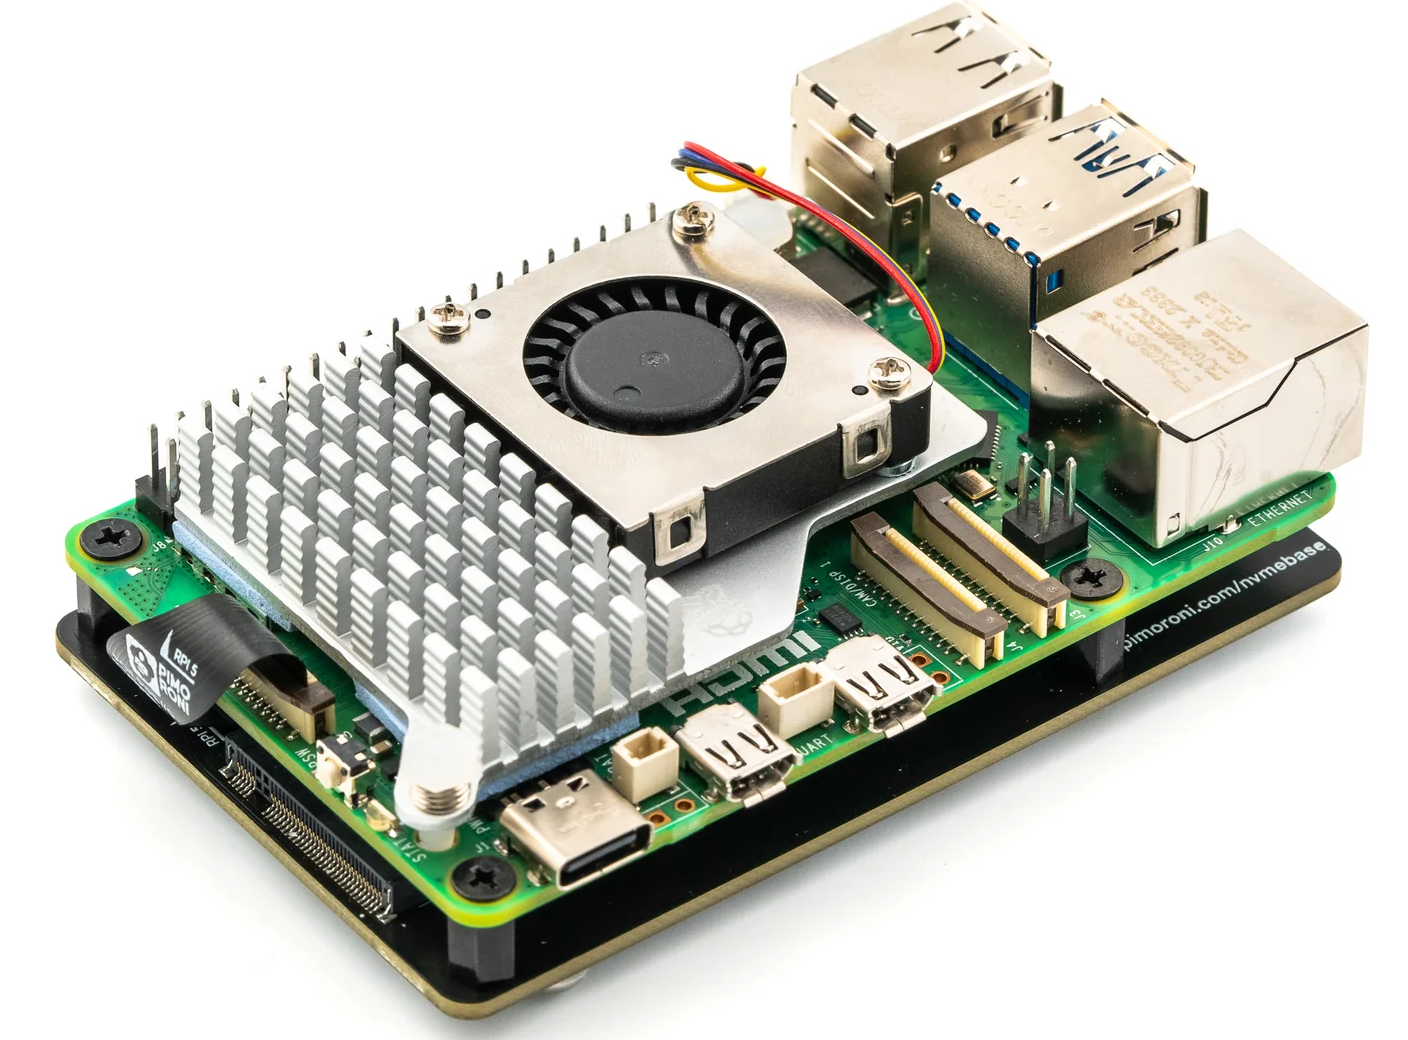
\includegraphics[width=0.3\textwidth]{nvmeRpi5.png}
    \caption{Raspberry Pi 5 with NVME SSD \cite{pimoroni_nvme_base}}
    \label{fig:Rpi5}
\end{figure}

As seen in Table \ref{tab:sbc_comparison}, the RPi5 has a quad-core ARM Cortex-A72 CPU, 8GB of LPDDR4-3200 SDRAM, and a 1Gbit Ethernet port. The RPi5 was chosen for its relatively low cost, small form factor, and wide range of software support. Other SBC's from Table \ref{tab:sbc_comparison} were considered, but the Rpi5 represented the best balance of performance and cost for the project, for example, the higher cost of the Nvidia Jetson was not justified for the project requirements. The viability of the Raspberry Pi5 in the context of testbed design and functionality was analysed based on the following points:

\noindent \textbf{Advantages}
\begin{itemize}
    \item \textbf{Storage:} The RPi5 supports external storage options via microSD, along with configurable HATs (hardware attached on top) for NVME SSDs, see section \ref{sec:storage} \cite{pimoroni_nvme_base}.
    \item \textbf{Size:} Its small form factor (85.6 x 56.5 mm) - roughly the size of a credit card, makes it easy to integrate into a testbed setup. Easily obtainable cooling fan.
    \item \textbf{GPIO:} 40 Pin GPIO header, can be used for interfacing with a prospective testbed user. Driven by the RP1 (custom I/O controller chip) \cite{core_electronics_rpi5}, the I/O is programmable with python.
    \item \textbf{Networking Capability:} Includes a 1Gbit Ethernet port and Wi-Fi 802.11ac, facilitating high-speed data transfer and network communication. Capable of 217.6 MB/s over Wi-Fi \cite{rpi5_wifi}.
    \item \textbf{Processing Capability:} Equipped with a quad-core ARM Cortex-A72 CPU and 8GB of LPDDR4-3200 RAM, enabling 2.4 GHz clock \cite{core_electronics_rpi5}.
    \item \textbf{Cost-Effectiveness:} Price of \$150 AUD, making it an affordable option for the project, approximately 1.5 the cost of the RPi4 (however almost double the performance) \cite{core_electronics_rpi5}
    \item \textbf{Software Support:} Extensive community support and availability of a wide range of software tools and libraries, especially for Linux-based systems, e.g. RTL-SDR, GNU Radio, etc. see section \ref{sec:SDRsoftware}.
\end{itemize}

\noindent \textbf{Disadvantages} \todo{Add to this as project preogresses}
\begin{itemize}
    \item \textbf{Limited Built-In Storage:} The built-in storage is minimal, so additional external storage is necessary for handling large volumes of data.
    \item \textbf{Performance Constraints:} While powerful, it may not handle very high-frequency or complex radar signal processing as efficiently as more specialized or high-performance computing platforms, custom algorithms potentially required \cite{IOTpassiveRadar}.
    \item \textbf{Heat Management:} Under continuous heavy load, the RPi5 may require additional cooling solutions to prevent overheating.
    \item \textbf{Limited I/O Bandwidth:} The available I/O bandwidth might be a bottleneck for applications requiring very high-speed data acquisition and processing.
    \item \textbf{Power Supply:} Requires a stable power supply of 5.1V / 15W; not ideal for potentially portable or battery-powered applications \cite{rpi5_wifi}. 
\end{itemize}



\subsection{NVME Based Storage \label{sec:storage}}
Following on from the selection and testing of the Raspberry Pi 5 as the testbed computing platform, it became evident that the default 32GB microSD card used to boot and run the operating system was insufficient for the storage requirements of the project. The chosen solution for the bottleneck was to utilise a NVME SSD drive, connected via PCIe to the Raspberry Pi 5, specifically the Pimoroni Base \cite{pimoroni_nvme_base}.

In order to compare and quantify the differences in the storage performance between the microSD card and the NVME SSD, a series of tests were conducted, utilising the following linux commands via the terminal of the RPi5.

\begin{verbatim}
    lsblk
    sudo hdparm -t --direct /dev/nvme0n1 
    sudo hdparm -t --direct /dev/mmcblk0
\end{verbatim}

\noindent Resulting in the following output seen below in Table \ref{tab:diskperf}.

\begin{table}[h!]
    \centering
    \caption{Disk Read Performance: NVMe vs MicroSD Card \label{tab:diskperf}}
    \begin{tabular}{|l|l|}
    \hline
    \textbf{Device} & \textbf{Read Performance} \\ \hline
    \texttt{NVMe SSD (\texttt{/dev/nvme0n1})} & \texttt{751.22 MB/sec} \\ \hline
    \texttt{MicroSD Card (\texttt{/dev/mmcblk0})} & \texttt{84.83 MB/sec} \\ \hline
    \end{tabular}
\end{table}

The results in Table \ref{tab:diskperf} clearly show the obtained significant performance increase when using the NVME SSD compared to the microSD card. Given the large amount of data that generated and processed during the SDR sampling. Further NVME SSD configuration details include: 

\begin{itemize}
    \item \textbf{File System:} The NVME SSD was formatted with the ext4 file system, which is the default file system for most Linux distributions. 
    \item \textbf{Mounting:} The NVME SSD was mounted to the RPi5 at the following location: \texttt{/mnt/nvme0n1}
    \item \textbf{Connector}: PCIe x4 interface Gen 2.0, which is a high-speed interface standard that is commonly used for connecting storage devices to a computer.
    \item \textbf{Supported NVMe Drives}: Supports M.2 NVMe drives (2280 size)
    \item \textbf{SSD Model:} Patriot P300 NVMe M.2 SSD, 128GB capacity, used for both storage and booting the RPi5.
\end{itemize}


\subsection{Antenna Configuration \label{sec:antenna}}
Intially, a simple SMA whip antenna was used for the RTL-SDR, as seen in Figure \ref{fig:rtlSDR}. These low cost antennas are typically used for general purpose reception, and are not optimised for any specific frequency range. The whip antenna was used for initial testing and prototyping, and was capable of receiving a range of broadcast signals with a NOISE FLOOR X. Eventually a more specialised antenna was used, the Yagi-Uda antenna, which is a directional antenna that is commonly used for point-to-point communication. The Yagi-Uda antenna was used for the final testing and validation of the testbed. The Yagi-Uda was utilised with a CLF200 50 Ohm coaxial cable, which was connected to the RTL-SDR. 

% IMAGE OF THE NOISE FLOOR COMPARISON


The physical setup of these antennas for testing comprised of an "Over the Shoulder" geometry whereby the antenna was placed behind a building in the line of sight of the TX signal (in this case Mt Cootha). For a single channel / antenna PBR setup, this geometry works to attenuate the direct path signal, and allow for the reflection to be better received by the antenna. 
\todo[inline]{diagram of geometry of map / antenna}

\subsubsection{Antenna Signal Strength Testing} \todo{Discuss what to do, put this in results}
Before calculations or detection was performed, the signal strength of the received signal was measured. This was done by first using the RTL-SDR and the monopole SMA antenna and compared to the Yagi-Uda antenna. The received signal strength, representing the illuminator DAB signal, was measured approximately 6km away from the transmitter tower. \todo{image of maps reference} The results of the signal strength measurements are shown in Table \ref{tab:signalstrength}.

\begin{table}[h!]
    \centering
    \caption{Noise Floor and SNR Comparison with -14.2 dB Gain (RTL-SDR)}
    \label{tab:signalstrength}
    \begin{tabular}{|c|c|c|c|}
        \hline
        \textbf{Antenna Type} & \textbf{Noise Floor (dB)} & \textbf{Signal Strength (dB)} & \textbf{SNR (dB)} \\ \hline
        SMA Monopole & -60 & -40.9 & 19.1 \\ \hline
        Yagi-Uda     & -60 & -17   & 43   \\ \hline
    \end{tabular}
    \vspace{0.5cm}
\end{table}

The above table reflects the high gain of the Yagi-Uda antenna, which is a directional antenna, compared to the monopole SMA antenna. Overall, this testing was valuable to benchmark a noise floor and appreciate the neccessity for a high gain antenna, especially in the context of the low power target signal.


\subsection{Testbed Design \label{sec:testbed}}
Building off the aforementioned hardware components, it was then necessary to develop a physical testbed setup that would allow for the SDR receiver module to be connected to the embedded computing platform, and for the entire system to be powered and networked. Also, given the scope of the project, it was necessary to have a protective encasing for the Rpi5 which also implemented user functionality (ie. pushbuttons and LED's). The testbed was designed to be portable and easily deployable, with the following key components and features:

\todo[inline]{ADD IMAGE OF TESTBED}

\begin{itemize}
    \item \textbf{Enclosure:} A custom 3D printed enclosure was designed to house the RPi5, the RTL-SDR, and the NVME SSD HAT seen in \ref{fig:Rpi5}. The enclosure was designed to be compact and portable, with a small form factor that could be easily transported and deployed in various environments. The enclosure was designed to be easily opened and closed, with a removable top panel that allowed for easy access to the internal components. The printed acrylic was also designed for cooling purposes, with ventilation holes on the top and sides of the enclosure to allow for airflow, bolstered by the Rpi5 active cooling fan and heatsink.
    \item \textbf{User Interface:} It was envisaged that the testbed have some sort of capability that would enable physical triggering of PBR sampling and processing \todo{REMOTE??}. Arcade style pushbuttons with LED's were selected to facilitate this interface \cite{pushbuttons}. The pushbuttons were connected to the GPIO pins of the RPi5, and were programmed to trigger the PBR sampling and processing functions (implemented via python scripts). The LED's were used to indicate the status of the PBR system, with different colours indicating different states of the system.
    \item \textbf{Power Supply:} A 5V / 15W power supply was used to power the RPi5, with a USB-C connector that allowed for easy connection to the RPi5. The power supply was connected to a power strip that allowed for multiple enclosures to be powered from a single power source.
    \item \textbf{Networking:} The ethernet port on the Rpi5 was left unobstructed by the case for potential wired networking. With the main focus of being geared towards Wi-Fi based networking which was all facilitated by the Rpi5 system on chip.\todo{network details}
    \item \textbf{Radio Front End:} It was intended for the SDR module to be connected via the USB 3.0 port with the enclosure not designed to house the SDR unit (for versatility). Per SDR functionality, the antenna was connected via coaxial cable, also not housed in the enclosure. 
    
\end{itemize}

In summary, the testbed was designed to be a portable, easily deployable system that could be used to test and validate the passive radar detection system. The enclosure was designed to house the RPi5, the NVME HAT, with the remaining system hardware components not specific to the testbed itself (possible to change out). This part of the project design was important for achieving the primary objectives, notably objective 2 as stated in \ref{sec:aims}.

\section{Software}

\subsection{SDR Software \label{sec:SDRsoftware}}
When utilising SDR modules, it is necessary to have capabilities to demodulate and then process the received signals. This is typically done using SDR software, which is a type of software that allows for the reception and baseband processing of radio signals using SDR hardware. For this project, the RTL-SDR was used in conjunction with the following software tools:


\subsection{Networking Requirements \label{sec:networking}}


% METHOD FOR TESTING NOT THE ACTUAL RESULTS
\section{Digital Signal Processing Testing \& Simulation}



